%author: Pedro Pinto; v2.5; jun 2020
\documentclass[11pt,a4paper]{report}
\usepackage{amsmath}
\usepackage{graphicx}
\usepackage{tabularx}
\usepackage{adjustbox}
%\usepackage[colorinlistoftodos]{todonotes}
\usepackage{csquotes}
\usepackage{comment}
\usepackage{imakeidx}
%tabela
\usepackage{multirow}
\usepackage{xcolor}
\usepackage[margin=3cm]{geometry}
\usepackage{hyperref}
\usepackage[toc,acronym,nopostdot,nonumberlist]{glossaries}
\usepackage{titling}
\usepackage{tikzpagenodes}
\usepackage[ddmmyyyy]{datetime}
\usepackage{setspace}
\usepackage{indentfirst}

%para definir a localização das tabelas e imagens em modo strict
%\usepackage{placeins}

\usepackage{biblatex}
\addbibresource{ref.bib}
\makeglossaries

%colocar aqui variáveis que serão utilizadas no texto:
\newcommand\kbps{\text{\textit{k}bit/s}}
\doublespacing

\begin{document}

\begin{titlepage}
\begin{tikzpicture}[remember picture,overlay,shift={(current page.center)}]
\node[anchor=center,xshift=0cm,yshift=9.5cm,opacity=0.75]{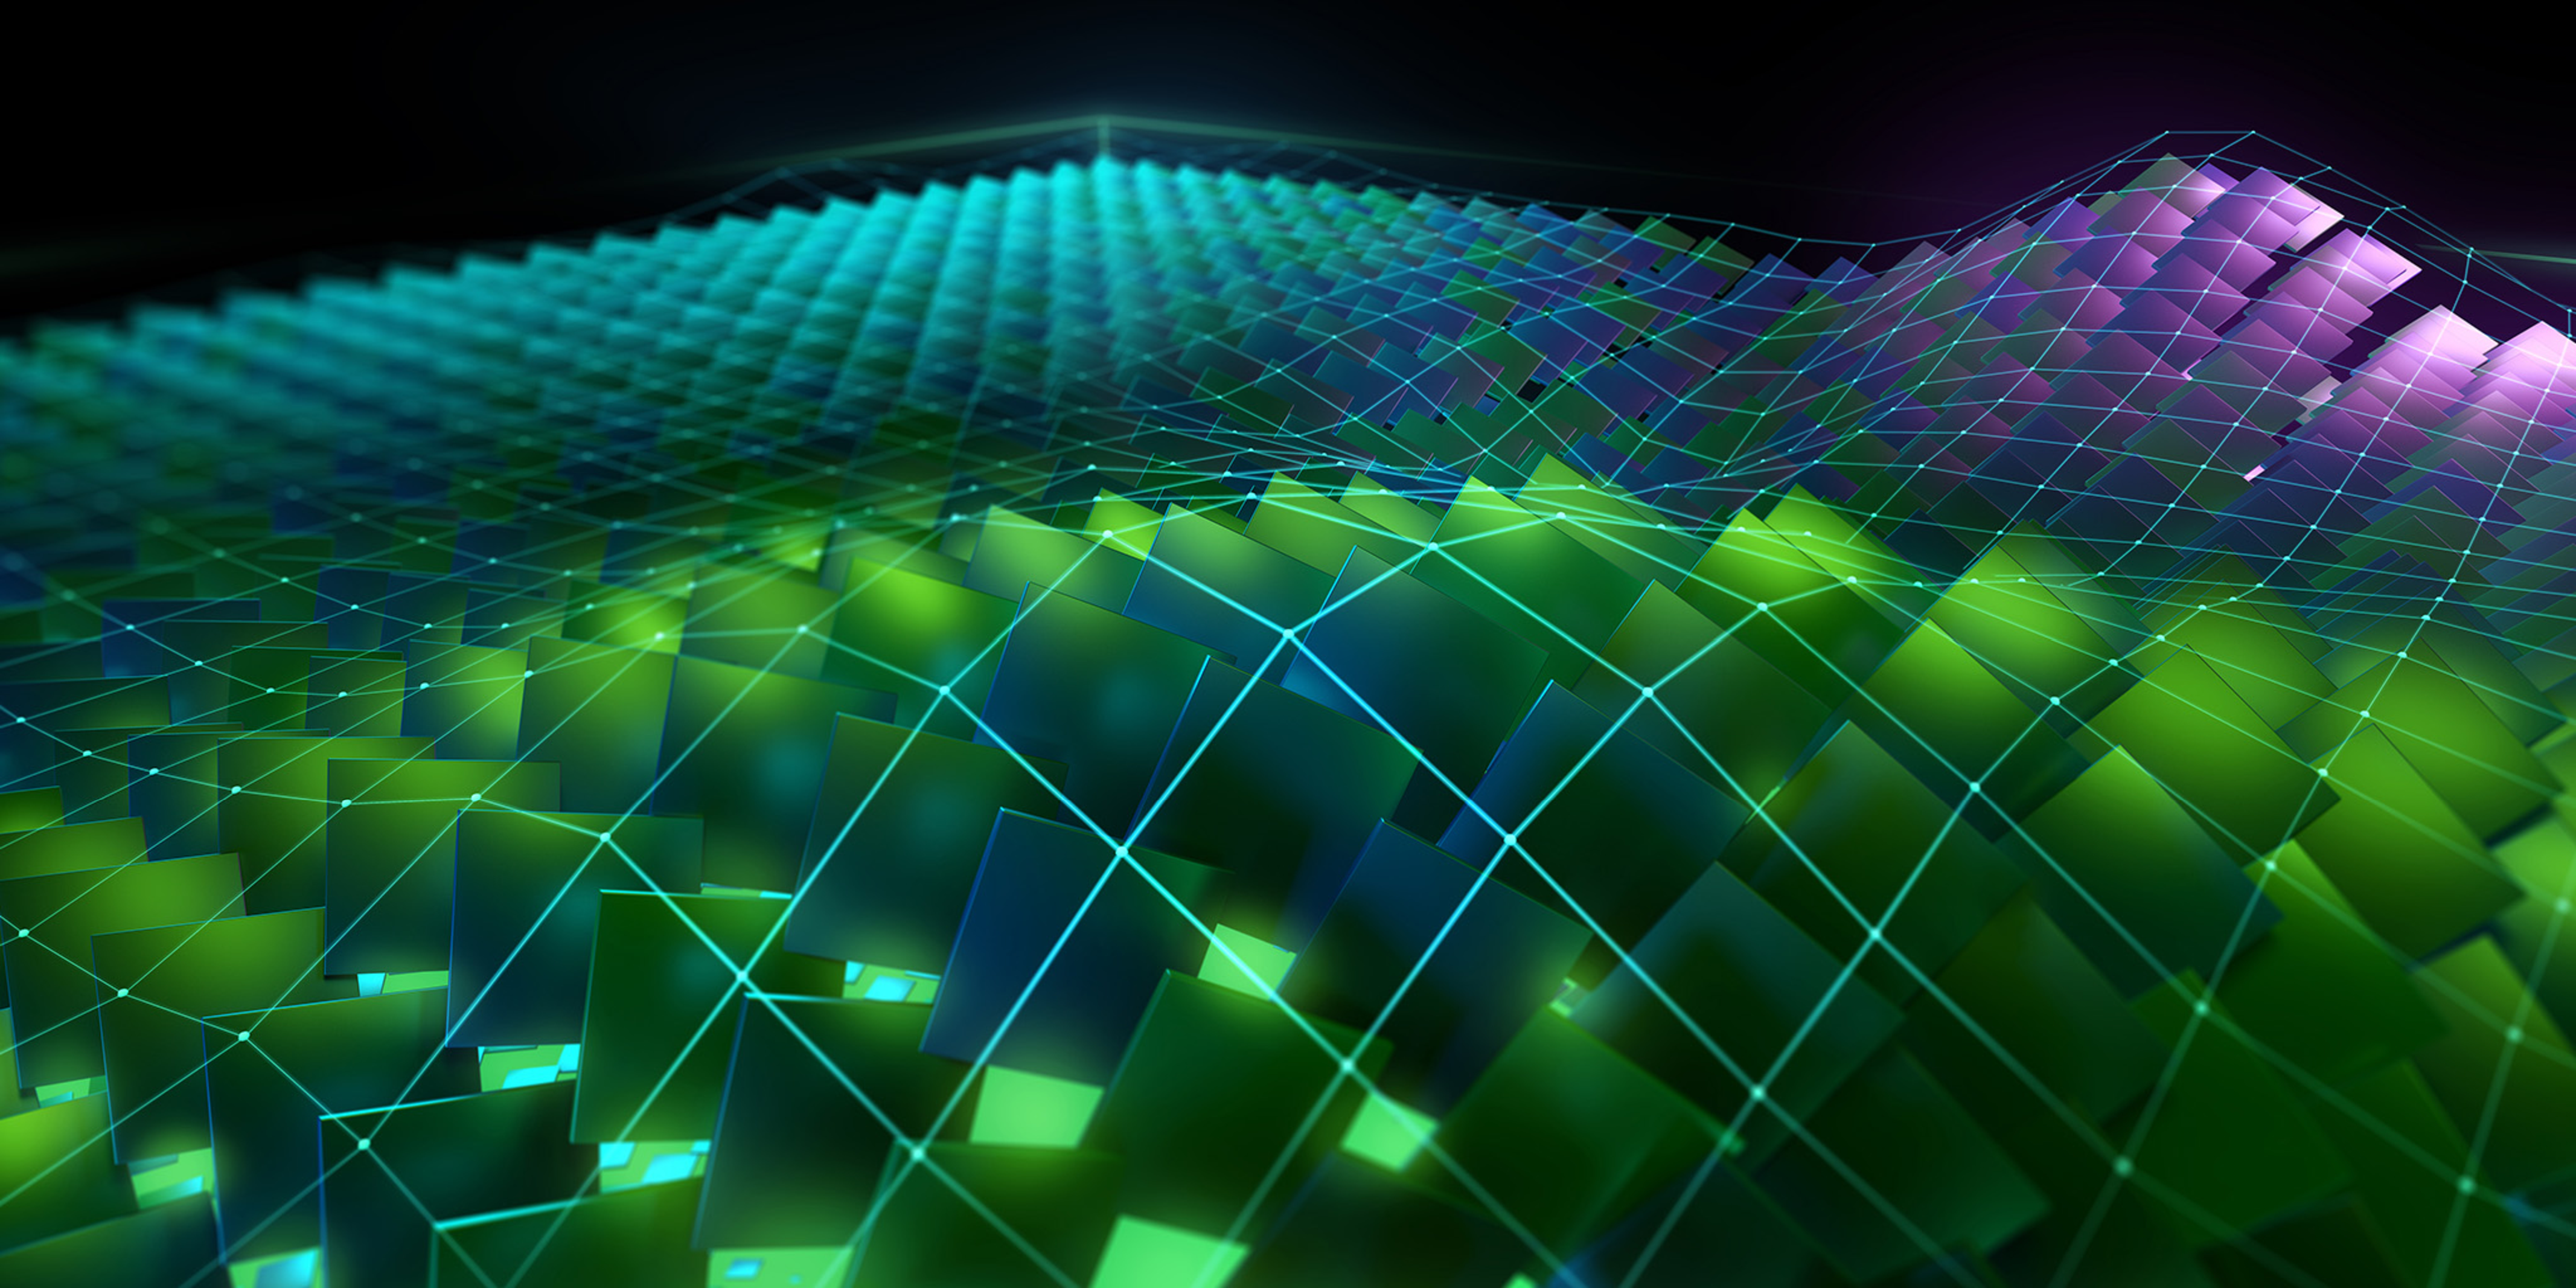
\includegraphics[scale=0.3]{figs/cuda-frontpage.pdf}};
\end{tikzpicture}

\centering
\vspace{10cm}
\huge Classifying CIFAR-10 with Transfer Learning and GPU Acceleration \\
\vspace{3cm}
\large A DD2360 Project\\
%\large a lab assignment report authored by\\
\Large Roderick Karlemstrand\\
\Large KTH Royal Institute of Technology \\

% \large supervised by\\
% %#if Project uncomment
% \large name\\

%#if Internship uncomment following lines
%\large Prof. X (ESTG-IPVC)\\
%\large Name of Company Supervisor (Company X)\\

\vspace{3cm}
%#if Internship uncomment following lines
%\includegraphics[scale=0.35]{figs/ESTG-IPVC.png}

\newdateformat{daymonthyear}{\THEDAY\ \monthname[\THEMONTH], \THEYEAR}
\daymonthyear\today \\
%December, 2019
%\large v2.3
\end{titlepage}

%%%% colocar aqui acrónimos
\newacronym{ersc}{ERSC}{Engenharia de Redes e Sistemas de Computadores}
\newacronym{wn}{WN}{Wireless Network}

%%%%%%%%%%%%%%%%%%%%%%%%%%%%%%%%%%%%%%%%%%%%%%%%%%%%%
\begin{abstract}
%context

%problem

%proposal

%solution

CIFAR-10 is a famous dataset for multiclassification problems. In this project, a Variational Autoencoder is used to classify an unlabel sub-dataset of CIFAR-10 of 10 000 elements. Next, a small labeled dataset is used to train the classification model. The model is lastly evaluated by a test dataset. The training process takes approximately 30 minutes per epoch with CPU, so that the whole training may take days to finish one experiment. To make the research possible, a GPU accelerated environment was implemented. The results shows a speedup by 10 times, and the classification accuracy is around 37\%. \\

\textbf{Keywords:} Image classification, Variational Autoencoder, Deep learning, Transfer Learning, GPU acceleration


\end{abstract}


%insert index
\tableofcontents
\glsaddall
\printglossary[type=\acronymtype]
\printglossary[type=main,title={Glossary},toctitle={Glossary}]
%%%%%%%%%%%%%%%%%%%%%%%%%%%%%%%%%%%%%%%%%%%%%%%%%%%%%

\chapter{Introduction}
\label{chap:introduction}

Computer vision is a field of study in Machine Learning, to give computer programs the ability to see. As for humans, the light reaches the retina and signals are then sent to the brain for further processing. Human brains can connect sight with other senses, like touch, sound or smell. This makes it easy to extract certain things from the sight, in order to identify them. For example, a child may recognise a bike after seeing a few of them. However, it is not easy for computer programs. The pictures is just like random numbers to them, and it would take thousands of training examples for a Machine Learning model to be able to identify one certain item.


\section{Problem Statement and Motivation}
\label{sec:motivation}

For supervised learning, the dataset has to be labeled and this is often done by humans. It is a very tedious and time-consuming job. Consider also another scenario that for automous driving cars, the comptuer program should be able to identify humans, objects, viheciles and many other things in the environment. And the input data is streaming. It would not be feasible to set labels on every one of these for every single frame. It may be possible to solve the problem in a more efficient way. In this project, a new learning algorithm of Transfer Learning is proposed. A VAE is used to seperate the unlabeled training dataset into 10 clusters. And a smalled labeled training dataset is used to help the model associate the clustered learnt with the correct labels. There are no misclassifications (i.e. noises in the dataset). In this way, the model may achieve the same prediction accuracy with much smaller labeled training dataset. The research questions are:

Is there a more efficient way of teaching computer programs to classify images without large labeled dataset?
How much faster does the training process run with a GPU, specifically Nvidia Tesla P100 16GB?


\section{Objectives}
\label{sec:name}

The objectives of this project is to build a VAE and transfer learning algorithm and to accelerate the training process with GPU.


\chapter{Methods}
\label{cap:method}

The design of the VAE and neural network is presented in this chapter. It also includes the dataset and training process.

\section{Variational Autoencoders}
\label{sec:vae}

A autoencoder is a type of neural network that tries to extract features from the input data and stores it in \textit{codes}. Codes is also known as abstract patterns. This technique forces the neural network to build a system to compress the data. Next, the code is fed into a decoder which tries to re-create the input data. The figure \ref{fig:vae}

\begin{figure}
\noindent\makebox[\textwidth]{%
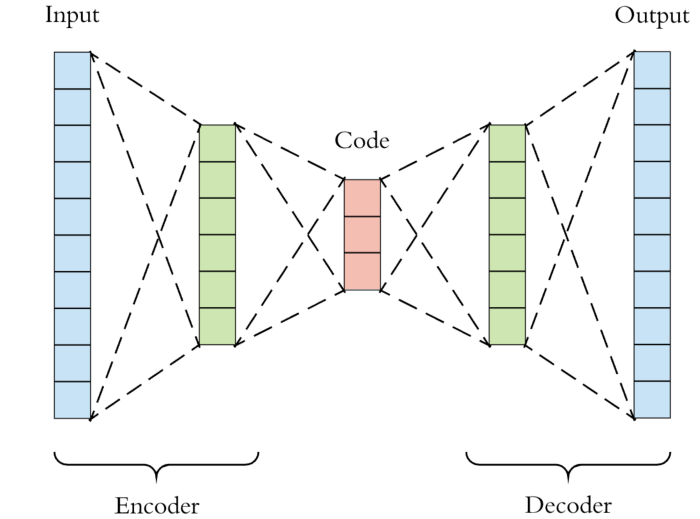
\includegraphics[width=0.8\textwidth]{figs/vae.png}}
\caption{An exampel of a Variational Autoencoder}
  \label{fig:vae}
\end{figure}

testtest

\begin{itemize}
    \item The quick brown fox jumps over the lazy dog. The quick brown fox jumps over the lazy dog. The quick brown fox jumps over the lazy dog. The quick brown fox jumps over the lazy dog. The quick brown fox jumps over the lazy dog. The quick brown fox jumps over the lazy dog.
    \item The quick brown fox jumps over the lazy dog. The quick brown fox jumps over the lazy dog. The quick brown fox jumps over the lazy dog. The quick brown fox jumps over the lazy dog. The quick brown fox jumps over the lazy dog. The quick brown fox jumps over the lazy dog.test
\end{itemize}

%%%%%%%%%%%%%%%%%%%%%%%%%%%%%%%%%%%%%%%%%%%%%%%%%%%%%
\chapter{Title of the chapter}
\label{cap:name2}

The quick brown fox jumps over the lazy dog. The quick brown fox jumps over the lazy dog. The quick brown fox jumps over the lazy dog. The quick brown fox jumps over the lazy dog. The quick brown fox jumps over the lazy dog. The quick brown fox jumps over the lazy dog.

\section{Section 2}
\label{sec:sec2}

The quick brown fox jumps over the lazy dog. The quick brown fox jumps over the lazy dog. The quick brown fox jumps over the lazy dog. The quick brown fox jumps over the lazy dog. The quick brown fox jumps over the lazy dog. The quick brown fox jumps over the lazy dog.


\addcontentsline{toc}{chapter}{References}
\printbibliography[title={References}]

\end{document}
